\documentclass[uplatex]{jsarticle}
\usepackage{url}
\usepackage{xurl}
\usepackage{amsmath,amsbsy}
\usepackage{amsthm}
\usepackage{bigints}
\usepackage[dvipdfmx]{graphicx}
\usepackage{bm}
\usepackage{physics} % physicsパッケージを読み込む
\usepackage{amsmath,amssymb}
\usepackage{mathtools}
\newcommand{\kakko}[1]{\left( #1 \right)}
\newcommand{\dec}[1]{\left\langle #1 \right\rangle}
\newcommand{\gauss}[1]{\left\lfloor #1 \right\rfloor}

\everymath{\displaystyle}
\usepackage{tikz}
\begin{document}
\title{明らかなこと,そうでないこと}
\author{mathtech会員}
\date{}
\maketitle
\newcommand{\R}{\mathbb{R}}
\newcommand{\N}{\mathbb{N}}
\newcommand{\Q}{\mathbb{Q}}
\newcommand{\Z}{\mathbb{Z}}
\newcommand{\C}{\mathbb{C}}
\newcommand{\st}{\sin \theta}
\newcommand{\ct}{\cos \theta}
\newtheorem{命題}{命題}
\newtheorem{thm}{thm}
\theoremstyle{definition}
\newtheorem{dfn}{Definition}
\newtheorem{definition}{Definition}
\newtheorem{fact}{Fact}




\section{はじめに}

数学において,自明とも言えるような主張をわざわざ証明することがよくある。
例えば,\\
\begin{itemize}
    \item 平面上に2点をとり、この2点を結ぶ連続な曲線を描く。そしてこの2点の位置関係が互いに反対側になるように直線を引いたとき、その曲線と直線とがどこかで必ず交点を持つ(中間値の定理)。
    \item 平面上の2点を結ぶなめらかな曲線を書けば、どこかで接線は2点を結ぶ線分に並行になる(平均値の定理)。
    \item 平面から輪っかを除くと平面は「内側」と「外側」に分かれる(ジョルダンの閉曲線定理)。
\end{itemize}

もちろんこれらは厳密な数学的な主張ではないので,主張自体は数学の言葉で書かれるが,
言っていることは上のようなことである。
\\
なぜこのようなことは自明で片付けては行けないのだろうか?
結論から言うと,直感はあてにならないことが多いからである。
それを示す一例について話そうと思う。

\section{2つの定理の感覚的な主張と数学的な主張}
今回話す2つの定理の数学的な主張をまず述べよう。

\begin{thm}\label{thm:injection}
    $
        \mathbb{R}^3から\mathbb{R}^2への単射連続写像は存在しない。
    $
\end{thm}

\begin{thm}\label{thm:surjection}
    $
        \mathbb{R}^2から\mathbb{R}^3への全射連続写像は存在する。
    $
\end{thm}
(連続性,単射,全射などの定義は
Definition\refeq{Def:continuity},\refeq{Def:injection},\refeq{Def:surjection}
を参照。)

では,次に定理の感覚的な言い換えをしよう。
thm\refeq{thm:injection} は,空間を2点が重ならないように平面に連続変形することができない事を言い,
thm\refeq{thm:surjection}は,平面を連続変形することで空間にできることを言う。

おそらく,thm\refeq{thm:injection}は明らかな主張に思えるが,
thm\refeq{thm:surjection}は直感に反する主張に思えるだろう。

そして,thm\refeq{thm:injection}の成立は簡単には行かない(と思われる)。\\
証明の道筋を述べるだけでも長くなるので,まずはthm\refeq{thm:surjection}を示して。
その後thm\refeq{thm:injection}の道筋を示そう。





\section{thm\refeq{thm:surjection}の証明}
直接\(\mathbb{R}^2から\mathbb{R}^3への全射連続写像を構成するのではなく,
まず線分から三角形領域への全射連続写像を構成し,その後\)thm\refeq{thm:surjection}を示そう。

\subsection{線分から三角形への写像の構成}
次にようにして0,1を結ぶ線分上の点をを平面の点に対応させる。
線分を\(L\)と表し,平面上の3点(1,0)(0.1)(0,-1)が成す直角2等辺三角形を\(T\)で表す。\\
まず,線分,三角形を2等分し,\(0, 1\)に対応付ける。
\(L,T\)はそれぞれ\(L_0,L_1,T_0,T_1\)に分けられる。
\tikzset{every picture/.style={line width=0.75pt}} %set default line width to 0.75pt        

\begin{tikzpicture}[x=0.75pt,y=0.75pt,yscale=-1,xscale=1]
    %uncomment if require: \path (0,300); %set diagram left start at 0, and has height of 300

    %Shape: Right Triangle [id:dp6960929835075491] 
    \draw   (247.39,34) -- (390.78,173.44) -- (247.39,173.44) -- cycle ;
    %Shape: Right Triangle [id:dp9026844503256424] 
    \draw   (247.39,34) -- (104,173.44) -- (247.39,173.44) -- cycle ;

    % Text Node
    \draw (192,119) node [anchor=north west][inner sep=0.75pt]   [align=left] {0};
    % Text Node
    \draw (289,118) node [anchor=north west][inner sep=0.75pt]   [align=left] {1};
    % Text Node
    \draw (314,181) node [anchor=north west][inner sep=0.75pt]   [align=left] {1};
    % Text Node
    \draw (176,181) node [anchor=north west][inner sep=0.75pt]   [align=left] {0};


\end{tikzpicture}


次に,先程分けた線分,三角形を再度2等分し,
\(00, 01, 10, 11\)に対応付ける。
\(L,T\)はそれぞれ\(L_{00},L_{01},L_{10},L_{11},T_{00},T_{01},T_{10},T_{11}\)に分けられる。\\
ここで,2進数で隣り合う01,10と対応する三角形\(T_{01},T_{10}\)が接していることに注意する。

\tikzset{every picture/.style={line width=0.75pt}} %set default line width to 0.75pt        

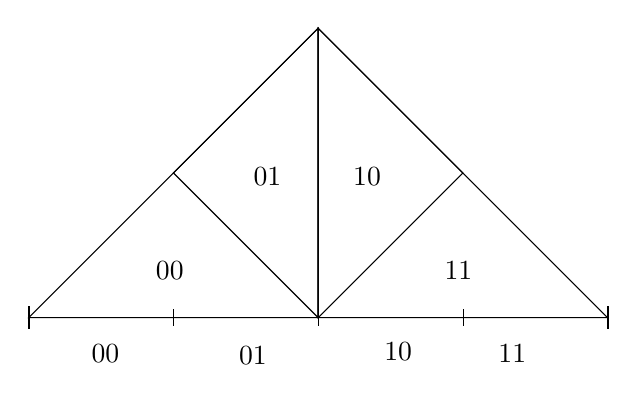
\begin{tikzpicture}[x=0.75pt,y=0.75pt,yscale=-1,xscale=1]
    %uncomment if require: \path (0,300); %set diagram left start at 0, and has height of 300

    %Shape: Right Triangle [id:dp6960929835075491] 
    \draw   (227.39,44) -- (366.83,183.44) -- (227.39,183.44) -- cycle ;
    %Shape: Right Triangle [id:dp4879420547761113] 
    \draw   (87.94,183.44) -- (227.39,44) -- (227.39,183.44) -- cycle ;
    %Shape: Right Triangle [id:dp5724350855741949] 
    \draw   (227.39,44) -- (227.39,183.44) -- (157.67,113.72) -- cycle ;
    %Shape: Right Triangle [id:dp2821099006540795] 
    \draw   (227.39,183.44) -- (227.39,44) -- (297.11,113.72) -- cycle ;
    %Straight Lines [id:da7404247155114849] 
    \draw    (87.94,183.44) -- (366.83,183.44) (157.74,179.44) -- (157.74,187.44)(227.54,179.44) -- (227.54,187.44)(297.34,179.44) -- (297.34,187.44) ;
    \draw [shift={(366.83,183.44)}, rotate = 180] [color={rgb, 255:red, 0; green, 0; blue, 0 }  ][line width=0.75]    (0,5.59) -- (0,-5.59)   ;
    \draw [shift={(87.94,183.44)}, rotate = 180] [color={rgb, 255:red, 0; green, 0; blue, 0 }  ][line width=0.75]    (0,5.59) -- (0,-5.59)   ;

    % Text Node
    \draw (148,155) node [anchor=north west][inner sep=0.75pt]   [align=left] {00};
    % Text Node
    \draw (117,195) node [anchor=north west][inner sep=0.75pt]   [align=left] {00};
    % Text Node
    \draw (195,110) node [anchor=north west][inner sep=0.75pt]   [align=left] {01};
    % Text Node
    \draw (243,110) node [anchor=north west][inner sep=0.75pt]   [align=left] {10};
    % Text Node
    \draw (188,196) node [anchor=north west][inner sep=0.75pt]   [align=left] {01};
    % Text Node
    \draw (258,194) node [anchor=north west][inner sep=0.75pt]   [align=left] {10};
    % Text Node
    \draw (287,155) node [anchor=north west][inner sep=0.75pt]   [align=left] {11};
    % Text Node
    \draw (313,195) node [anchor=north west][inner sep=0.75pt]   [align=left] {11};


\end{tikzpicture}

更に,先程分けた線分,三角形を再度2等分し,
\(000, 001, 010, 011, 100, 101, 110, 111\)に対応付ける。
\(L,T\)は上と同様に添字に8つの数字を対応させて分ける。\\
ここで,2進数で隣り合う\(001, 010\)と対応する三角形\(T_{001},T_{010}\)が接していることに注意する。
同じく,2進数が隣り合う\(011, 100\)と対応する三角形\(T_{011},T_{100}\)も接し,
\(101, 110\)と対応する三角形\(T_{101},T_{110}\)も接していることに注意せよ。
\tikzset{every picture/.style={line width=0.75pt}} %set default line width to 0.75pt        

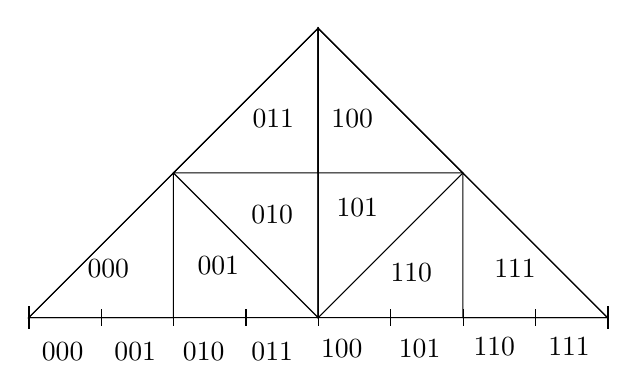
\begin{tikzpicture}[x=0.75pt,y=0.75pt,yscale=-1,xscale=1]
    %uncomment if require: \path (0,300); %set diagram left start at 0, and has height of 300

    %Shape: Right Triangle [id:dp8512969328948343] 
    \draw   (227.39,44) -- (366.83,183.44) -- (227.39,183.44) -- cycle ;
    %Shape: Right Triangle [id:dp37198217404572653] 
    \draw   (87.94,183.44) -- (227.39,44) -- (227.39,183.44) -- cycle ;
    %Shape: Right Triangle [id:dp8471781454068721] 
    \draw   (227.39,44) -- (227.39,183.44) -- (157.67,113.72) -- cycle ;
    %Shape: Right Triangle [id:dp851510091754339] 
    \draw   (227.39,183.44) -- (227.39,44) -- (297.11,113.72) -- cycle ;
    %Straight Lines [id:da06879509263800254] 
    \draw    (87.94,183.44) -- (366.83,183.44) (122.84,179.44) -- (122.84,187.44)(157.74,179.44) -- (157.74,187.44)(192.64,179.44) -- (192.64,187.44)(227.54,179.44) -- (227.54,187.44)(262.44,179.44) -- (262.44,187.44)(297.34,179.44) -- (297.34,187.44)(332.24,179.44) -- (332.24,187.44) ;
    \draw [shift={(366.83,183.44)}, rotate = 180] [color={rgb, 255:red, 0; green, 0; blue, 0 }  ][line width=0.75]    (0,5.59) -- (0,-5.59)   ;
    \draw [shift={(87.94,183.44)}, rotate = 180] [color={rgb, 255:red, 0; green, 0; blue, 0 }  ][line width=0.75]    (0,5.59) -- (0,-5.59)   ;
    %Shape: Right Triangle [id:dp10432328350335895] 
    \draw   (227.39,44) -- (297.11,113.72) -- (227.39,113.72) -- cycle ;
    %Shape: Right Triangle [id:dp614437626173427] 
    \draw   (297.11,113.72) -- (366.83,183.44) -- (297.11,183.44) -- cycle ;
    %Shape: Right Triangle [id:dp9197424591110392] 
    \draw   (157.67,113.72) -- (227.39,44) -- (227.39,113.72) -- cycle ;
    %Shape: Right Triangle [id:dp15344254461964435] 
    \draw   (87.94,183.44) -- (157.67,113.72) -- (157.67,183.44) -- cycle ;

    % Text Node
    \draw (115,154) node [anchor=north west][inner sep=0.75pt]   [align=left] {000};
    % Text Node
    \draw (128,194) node [anchor=north west][inner sep=0.75pt]   [align=left] {001};
    % Text Node
    \draw (161,194) node [anchor=north west][inner sep=0.75pt]   [align=left] {010};
    % Text Node
    \draw (232.53,81.86) node [anchor=north west][inner sep=0.75pt]   [align=left] {100};
    % Text Node
    \draw (194.53,81.86) node [anchor=north west][inner sep=0.75pt]   [align=left] {011};
    % Text Node
    \draw (235,125) node [anchor=north west][inner sep=0.75pt]   [align=left] {101};
    % Text Node
    \draw (261,156) node [anchor=north west][inner sep=0.75pt]   [align=left] {110};
    % Text Node
    \draw (311,154) node [anchor=north west][inner sep=0.75pt]   [align=left] {111};
    % Text Node
    \draw (93,194) node [anchor=north west][inner sep=0.75pt]   [align=left] {000};
    % Text Node
    \draw (168,153) node [anchor=north west][inner sep=0.75pt]   [align=left] {001};
    % Text Node
    \draw (194,128) node [anchor=north west][inner sep=0.75pt]   [align=left] {010};
    % Text Node
    \draw (227.53,192.86) node [anchor=north west][inner sep=0.75pt]   [align=left] {100};
    % Text Node
    \draw (194,194) node [anchor=north west][inner sep=0.75pt]   [align=left] {011};
    % Text Node
    \draw (265,193) node [anchor=north west][inner sep=0.75pt]   [align=left] {101};
    % Text Node
    \draw (301,192) node [anchor=north west][inner sep=0.75pt]   [align=left] {110};
    % Text Node
    \draw (337,192) node [anchor=north west][inner sep=0.75pt]   [align=left] {111};


\end{tikzpicture}

同様な操作を繰り返し,nステップ目でTを\(2^n\)つに分けて,
2進数で隣り合う数に対応する三角形が接するように三角形に数を対応させる。
\\
ではこのように作った三角形\(T_{i_1i_2i_3\cdots }\)を用いて,
\(LからT\)への写像を構成する。

\(L\)=[0,1](0,1を繋ぐ線分)上の点tに対し,それを2進数で小数展開することで,
\(t=0.i_1i_2i_3\cdots\)と表そう。\\
(小数展開が一意でないこと,またt=1のときにどうするかは後述,
ともかく小数展開できることが重要である)
このtに対し,
縮小する三角形の列
\(T_{i_1}\supset T_{i_1i_2}\supset T_{i_1i_2i_3},\supset \cdots \)
を考える。この列はただ1つの共有点を定めるから,その点を\(f(t)\)と定める。
この\( f:L\to T \)が全射で連続であること
(また小数展開の多意性によるwell-defined性の問題等)を示す。

\subsection{\(f\)がwell-defined であること}
\(fはtを小数展開してf(t)を定めたので,tの小数展開によってf(t)が変わってしまうと困る。\\
例えば,0.100\cdots =0.111\cdots であるが,このときに
f(0.100\cdots )=f(0.111\cdots) であるだろうか?\\
これは正しい,それは次のように示される。\\
f(0.100\cdots )は
T_{1}\supset T_{10}\supset T_{100},\supset \cdots
の共有点である。一方\\
f(0.011\cdots )は
T_{0}\supset T_{01}\supset T_{011},\supset \cdots
の共有点となる。ここで,2進数として隣り合う三角形は接する
(そのようにLを分けた)ことを思い出すと,
f(0.100\cdots ),f(0.011\cdots )は共に縮小する線分の列
T_{1}\cap T_{0}\supset T_{10}\cap T_{01}\supset T_{100}\cap T_{011},\supset \cdots
の共有点となる。
これより,f(0.100\cdots )=f(0.011\cdots )
を得る。\\
他の場合,つまり2進数が有限小数として止まりうる場合も,
同様にして示すことができる。
また,1は0.111\cdots とみなしてf(1)はf(0.111\cdots)のこととする。
これでfが上手く定まる(well-definedとなる)ことがわかった。
\)


\subsection{\(f\)が連続であること}
\(
これは,任意の\varepsilon を取ってt,t'の差を十分小さくすれば,
f(t)とf(t')の差が十分小さくなることを示せばよいが,
それは次にようにして分かる。
\)

\begin{thm}\label{thm:continuity of f}
    $
        \abs*{t-t'}<2^{-n}ならば\abs*{f(t)-f(t')}\leqq 2^{-n+2}
    $
\end{thm}
\begin{proof}
    \(
    分割のnステップにおいてLは2^{-n}つに分割される。
    この分割の下,t,t'は同じ線分に入るか隣り合う線分に入るかのどちらかであるから,
    (\because そうでない,つまり1つ以上飛んだ線分に入っているとすれば
    線分の長さが2^{-n}であるから\abs*{t-t'}>2^{-n}でなければならない。
    それは\abs*{t-t'}<2^{-n}に反する)
    f(t)とf(t')は線分と対応する三角形に属するので,
    同じ,もしくは隣り合う三角形に属することが分かる。
    下図より,最も離れる場合を考えても,
    \abs*{f(t)-f(-t)}\leqq 2^{-n+2}
    であるから,目的の不等式を得る。
    \)
\end{proof}

\tikzset{every picture/.style={line width=0.75pt}} %set default line width to 0.75pt        

\begin{tikzpicture}[x=0.75pt,y=0.75pt,yscale=-1,xscale=1]
    %uncomment if require: \path (0,300); %set diagram left start at 0, and has height of 300

    %Shape: Right Triangle [id:dp2851165540479339] 
    \draw   (231.39,108) -- (301.11,177.72) -- (231.39,177.72) -- cycle ;
    %Shape: Right Triangle [id:dp21221847705726993] 
    \draw   (161.67,177.72) -- (231.39,108) -- (231.39,177.72) -- cycle ;
    %Shape: Right Triangle [id:dp836744242199637] 
    \draw   (367.39,110) -- (437.11,179.72) -- (367.39,179.72) -- cycle ;
    %Shape: Right Triangle [id:dp3280432179367443] 
    \draw   (437.11,179.72) -- (367.39,110) -- (437.11,110) -- cycle ;
    %Curve Lines [id:da9833959735628928] 
    \draw  [dash pattern={on 0.84pt off 2.51pt}]  (190.78,217.22) .. controls (173.23,207.47) and (173.74,206.28) .. (162.65,185.83) ;
    \draw [shift={(161.78,184.22)}, rotate = 61.39] [color={rgb, 255:red, 0; green, 0; blue, 0 }  ][line width=0.75]    (10.93,-3.29) .. controls (6.95,-1.4) and (3.31,-0.3) .. (0,0) .. controls (3.31,0.3) and (6.95,1.4) .. (10.93,3.29)   ;
    %Straight Lines [id:da6726632282471039] 
    \draw    (231.39,110) -- (231.39,175.72) ;
    \draw [shift={(231.39,177.72)}, rotate = 270] [color={rgb, 255:red, 0; green, 0; blue, 0 }  ][line width=0.75]    (10.93,-3.29) .. controls (6.95,-1.4) and (3.31,-0.3) .. (0,0) .. controls (3.31,0.3) and (6.95,1.4) .. (10.93,3.29)   ;
    \draw [shift={(231.39,108)}, rotate = 90] [color={rgb, 255:red, 0; green, 0; blue, 0 }  ][line width=0.75]    (10.93,-3.29) .. controls (6.95,-1.4) and (3.31,-0.3) .. (0,0) .. controls (3.31,0.3) and (6.95,1.4) .. (10.93,3.29)   ;
    %Curve Lines [id:da10352101247510381] 
    \draw    (163.16,179.2) .. controls (173.62,189.14) and (182.99,188.36) .. (208.78,191.22) ;
    \draw [shift={(161.67,177.72)}, rotate = 45.99] [color={rgb, 255:red, 0; green, 0; blue, 0 }  ][line width=0.75]    (10.93,-3.29) .. controls (6.95,-1.4) and (3.31,-0.3) .. (0,0) .. controls (3.31,0.3) and (6.95,1.4) .. (10.93,3.29)   ;
    %Shape: Boxed Bezier Curve [id:dp9597654868376422] 
    \draw  [dash pattern={on 0.84pt off 2.51pt}]  (264.11,218.72) .. controls (284.08,208.97) and (283.5,207.78) .. (296.11,187.33) ;
    \draw [shift={(297.11,185.72)}, rotate = 121.83] [color={rgb, 255:red, 0; green, 0; blue, 0 }  ][line width=0.75]    (10.93,-3.29) .. controls (6.95,-1.4) and (3.31,-0.3) .. (0,0) .. controls (3.31,0.3) and (6.95,1.4) .. (10.93,3.29)   ;
    %Shape: Boxed Bezier Curve [id:dp7549672572922184] 
    \draw    (299.95,179.43) .. controls (290.71,192.53) and (282.52,191.49) .. (259.78,195.22) ;
    \draw [shift={(301.11,177.72)}, rotate = 123.18] [color={rgb, 255:red, 0; green, 0; blue, 0 }  ][line width=0.75]    (10.93,-3.29) .. controls (6.95,-1.4) and (3.31,-0.3) .. (0,0) .. controls (3.31,0.3) and (6.95,1.4) .. (10.93,3.29)   ;

    % Text Node
    \draw (155.89,43.29) node [anchor=north west][inner sep=0.75pt]  [font=\footnotesize]  {$ \begin{array}{l}
                t,t'は同じ,もしくは隣り合う線分に入るので, \\
                f( t) ,f( t') も同じ,もしくは隣り合う( 接する) 三角形に属する
            \end{array}$};
    % Text Node
    \draw (155.89,88.29) node [anchor=north west][inner sep=0.75pt]  [font=\footnotesize]  {$隣り合う( 接する) 三角形は次の2通りのみ$};
    % Text Node
    \draw (202.67,128.29) node [anchor=north west][inner sep=0.75pt]  [font=\tiny]  {$\frac{1}{2^{n-1}}$};
    % Text Node
    \draw (222.67,181.29) node [anchor=north west][inner sep=0.75pt]  [font=\tiny]  {$\frac{1}{2^{n-2}}$};
    % Text Node
    \draw (169.67,230.29) node [anchor=north west][inner sep=0.75pt]  [font=\footnotesize]  {$ \begin{array}{l}
                2点f( t) ,f( t) が最も離れるのはこの2点 \\
                つまり差は2^{-n+2} で抑えられる。
            \end{array}$};


\end{tikzpicture}
\((この証明は参考文献\cite{takagi}に準じた)\\
\text{thm}\refeq{thm:continuity of f}の成立から,fの連続性が従う。
それは,
任意の\forall \varepsilon > 0に対して
\varepsilon > 2^{-n+2}なるnを取り,
\delta を2^{-n}とすれば良いからである。
\)


\subsection{fが全射であること}
\(
任意の三角形の点Pに対し,対応する(つまりP=f(t)なる)tが存在することを示せばよいが,
分割の定義より三角形の点はnステップ目に必ずどこか(一つとは限らないが)の三角形に属する。\\
そのような三角形の列は減少列になるよう取れば(取ることができる),
その列
T_{i_1}\supset T_{i_1i_2}\supset T_{i_1i_2i_3}\supset
\cdots \supset T_{i_1i_2i_3\cdots }
が定めるi_1,i_2,i_3\cdots を用いて,
tを0.i_1i_2i_3\cdots と定めることで,定義から
f(t)=(減少列T_{i_1}\supset T_{i_1i_2}\supset T_{i_1i_2i_3}\supset
\cdots \supset T_{i_1i_2i_3\cdots }がが定めるただ一つの共有点)
=P
を得る。故にfは全射である。
\)

\subsection{直線から平面への連続全射の構成}

\(
では,fを用いて
\mathbb{R}から\mathbb{R}^2への連続全射\phi を構成しよう
\phi は次にように定めれば良い,(下図参照)。\\
0以下のxに対しては常に(-1,0)を取り
0から1で先程構成したfを用いて三角形領域を塗る。
1から2で2つ目で点を移動させ,
2から3でより大きい三角形を塗る,
3から4で再度移動して,
4から5でより大きい三角形を塗れば良い。
このようにして\phi を定めれば,これは平面全体を塗るだろう。
\)

\tikzset{every picture/.style={line width=0.75pt}} %set default line width to 0.75pt        

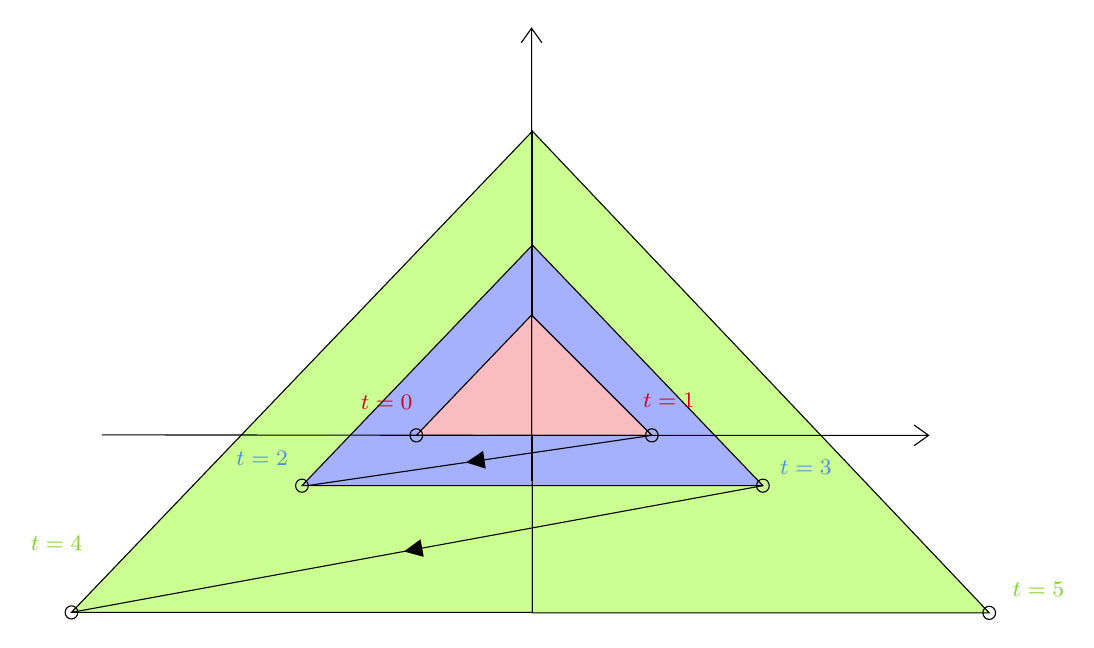
\begin{tikzpicture}[x=0.75pt,y=0.75pt,yscale=-1,xscale=1]
    %uncomment if require: \path (0,300); %set diagram left start at 0, and has height of 300

    %Shape: Right Triangle [id:dp2873907071874242] 
    \draw  [fill={rgb, 255:red, 203; green, 255; blue, 146 }  ,fill opacity=1 ] (107.94,293.44) -- (330.03,61.62) -- (330.03,293.44) -- cycle ;
    %Shape: Right Triangle [id:dp7763962515444283] 
    \draw  [fill={rgb, 255:red, 165; green, 177; blue, 253 }  ,fill opacity=1 ] (218.99,232.39) -- (330.03,116.48) -- (330.03,232.39) -- cycle ;
    %Shape: Right Triangle [id:dp340119113612394] 
    \draw  [fill={rgb, 255:red, 249; green, 188; blue, 193 }  ,fill opacity=1 ] (274.09,208.16) -- (329.61,150.2) -- (329.61,208.16) -- cycle ;
    %Straight Lines [id:da9663017923012163] 
    \draw    (329.61,208.16) -- (122.54,207.92) ;
    %Shape: Right Triangle [id:dp06090129586573534] 
    \draw  [fill={rgb, 255:red, 203; green, 255; blue, 146 }  ,fill opacity=1 ] (330.03,61.62) -- (550.11,293.67) -- (330.03,293.67) -- cycle ;
    %Shape: Right Triangle [id:dp5597818041110956] 
    \draw  [fill={rgb, 255:red, 165; green, 177; blue, 253 }  ,fill opacity=1 ] (330.03,116.48) -- (441.07,232.39) -- (330.03,232.39) -- cycle ;
    %Shape: Right Triangle [id:dp46851290909923926] 
    \draw  [fill={rgb, 255:red, 249; green, 188; blue, 193 }  ,fill opacity=1 ] (329.61,150.2) -- (387.57,208.16) -- (329.61,208.16) -- cycle ;
    %Straight Lines [id:da014864113301157333] 
    \draw    (107.94,293.44) -- (441.07,232.39) ;
    \draw [shift={(268.11,264.09)}, rotate = 349.61] [fill={rgb, 255:red, 0; green, 0; blue, 0 }  ][line width=0.08]  [draw opacity=0] (8.93,-4.29) -- (0,0) -- (8.93,4.29) -- cycle    ;
    %Shape: Axis 2D [id:dp6742682649907845] 
    \draw  (308.36,208.16) -- (520.9,208.16)(329.61,12) -- (329.61,229.95) (513.9,203.16) -- (520.9,208.16) -- (513.9,213.16) (324.61,19) -- (329.61,12) -- (334.61,19)  ;
    %Straight Lines [id:da7296650725909084] 
    \draw    (221.42,232.39) -- (387.57,208.16) ;
    \draw [shift={(298.06,221.21)}, rotate = 351.7] [fill={rgb, 255:red, 0; green, 0; blue, 0 }  ][line width=0.08]  [draw opacity=0] (8.93,-4.29) -- (0,0) -- (8.93,4.29) -- cycle    ;
    %Flowchart: Connector [id:dp2821436098079326] 
    \draw   (271.04,208.16) .. controls (271.04,206.41) and (272.4,204.99) .. (274.09,204.99) .. controls (275.78,204.99) and (277.15,206.41) .. (277.15,208.16) .. controls (277.15,209.91) and (275.78,211.32) .. (274.09,211.32) .. controls (272.4,211.32) and (271.04,209.91) .. (271.04,208.16) -- cycle ;
    %Flowchart: Connector [id:dp47696390013455714] 
    \draw   (215.93,232.39) .. controls (215.93,230.64) and (217.3,229.23) .. (218.99,229.23) .. controls (220.67,229.23) and (222.04,230.64) .. (222.04,232.39) .. controls (222.04,234.14) and (220.67,235.56) .. (218.99,235.56) .. controls (217.3,235.56) and (215.93,234.14) .. (215.93,232.39) -- cycle ;
    %Flowchart: Connector [id:dp49720375554938445] 
    \draw   (384.51,208.16) .. controls (384.51,206.41) and (385.88,204.99) .. (387.57,204.99) .. controls (389.26,204.99) and (390.62,206.41) .. (390.62,208.16) .. controls (390.62,209.91) and (389.26,211.32) .. (387.57,211.32) .. controls (385.88,211.32) and (384.51,209.91) .. (384.51,208.16) -- cycle ;
    %Flowchart: Connector [id:dp17628696276768352] 
    \draw   (438.01,232.39) .. controls (438.01,230.64) and (439.38,229.23) .. (441.07,229.23) .. controls (442.76,229.23) and (444.13,230.64) .. (444.13,232.39) .. controls (444.13,234.14) and (442.76,235.56) .. (441.07,235.56) .. controls (439.38,235.56) and (438.01,234.14) .. (438.01,232.39) -- cycle ;
    %Flowchart: Connector [id:dp5438161002106656] 
    \draw   (547.06,293.67) .. controls (547.06,291.92) and (548.42,290.5) .. (550.11,290.5) .. controls (551.8,290.5) and (553.17,291.92) .. (553.17,293.67) .. controls (553.17,295.42) and (551.8,296.83) .. (550.11,296.83) .. controls (548.42,296.83) and (547.06,295.42) .. (547.06,293.67) -- cycle ;
    %Flowchart: Connector [id:dp5932136475805974] 
    \draw   (104.89,293.44) .. controls (104.89,291.7) and (106.26,290.28) .. (107.94,290.28) .. controls (109.63,290.28) and (111,291.7) .. (111,293.44) .. controls (111,295.19) and (109.63,296.61) .. (107.94,296.61) .. controls (106.26,296.61) and (104.89,295.19) .. (104.89,293.44) -- cycle ;

    % Text Node
    \draw (246.11,187.67) node [anchor=north west][inner sep=0.75pt]  [font=\footnotesize,color={rgb, 255:red, 208; green, 2; blue, 27 }  ,opacity=1 ]  {$t=0$};
    % Text Node
    \draw (382.11,186.67) node [anchor=north west][inner sep=0.75pt]  [font=\footnotesize,color={rgb, 255:red, 208; green, 2; blue, 27 }  ,opacity=1 ]  {$t=1$};
    % Text Node
    \draw (186.11,214.67) node [anchor=north west][inner sep=0.75pt]  [font=\footnotesize,color={rgb, 255:red, 74; green, 144; blue, 226 }  ,opacity=1 ]  {$t=2$};
    % Text Node
    \draw (448.11,218.67) node [anchor=north west][inner sep=0.75pt]  [font=\footnotesize,color={rgb, 255:red, 74; green, 144; blue, 226 }  ,opacity=1 ]  {$t=3$};
    % Text Node
    \draw (87.11,255.67) node [anchor=north west][inner sep=0.75pt]  [font=\footnotesize,color={rgb, 255:red, 126; green, 211; blue, 33 }  ,opacity=1 ]  {$t=4$};
    % Text Node
    \draw (560.11,277.67) node [anchor=north west][inner sep=0.75pt]  [font=\footnotesize,color={rgb, 255:red, 126; green, 211; blue, 33 }  ,opacity=1 ]  {$t=5$};


\end{tikzpicture}


\subsection{平面から空間への連続全射の構成}
最後に,\(\mathbb{R}^2から\mathbb{R}^3への連続全射\psi を構成\)する。
\(
\mathbb{R}から\mathbb{R}^2への連続全射\phi を用いればそれは簡単で,
\psi(x,y)\coloneqq (x,\phi(y))とすれば良い。
各x_0\in \mathbb{R}に対し,yが直線x=x_0上を動くことで,
(x,\phi(y))は平面x=x_0全体を塗る。
よってx_0が\mathbb{R}全体を渡ることで(x,\phi(y))
は\mathbb{R}^3全体を渡るだろう。
\)

これで,
\(
\mathbb{R}^2から\mathbb{R}^3への連続全射を構成できた。
\phi と \psi の合成写像を考えれば,
\mathbb{R}から\mathbb{R}^3への連続全射も構成できる。
同様に考えれば
\mathbb{R}から\mathbb{R}^nへの連続全射も構成できる。
\)




\tikzset{every picture/.style={line width=0.75pt}} %set default line width to 0.75pt        

\begin{tikzpicture}[x=0.75pt,y=0.75pt,yscale=-1,xscale=1]
    %uncomment if require: \path (0,300); %set diagram left start at 0, and has height of 300

    %Shape: Axis 2D [id:dp24804142727471135] 
    \draw  (348.89,103.39) -- (444,103.39)(358.4,16.89) -- (358.4,113) (437,98.39) -- (444,103.39) -- (437,108.39) (353.4,23.89) -- (358.4,16.89) -- (363.4,23.89)  ;
    %Straight Lines [id:da5850418876890229] 
    \draw    (112.89,95) -- (215,95.98) ;
    \draw [shift={(217,96)}, rotate = 180.55] [color={rgb, 255:red, 0; green, 0; blue, 0 }  ][line width=0.75]    (10.93,-3.29) .. controls (6.95,-1.4) and (3.31,-0.3) .. (0,0) .. controls (3.31,0.3) and (6.95,1.4) .. (10.93,3.29)   ;
    %Shape: Axis 2D [id:dp08105781835670167] 
    \draw  (94.89,214.39) -- (190,214.39)(104.4,127.89) -- (104.4,224) (183,209.39) -- (190,214.39) -- (183,219.39) (99.4,134.89) -- (104.4,127.89) -- (109.4,134.89)  ;
    %Curve Lines [id:da6693493631086691] 
    \draw  [dash pattern={on 0.84pt off 2.51pt}]  (211.89,70) .. controls (248.26,51.38) and (301.06,51.97) .. (336.1,70.82) ;
    \draw [shift={(338.22,72)}, rotate = 209.74] [fill={rgb, 255:red, 0; green, 0; blue, 0 }  ][line width=0.08]  [draw opacity=0] (8.93,-4.29) -- (0,0) -- (8.93,4.29) -- cycle    ;
    %Shape: Axis 2D [id:dp5985126218634429] 
    \draw  (343.89,227) -- (443.89,227)(353.89,137) -- (353.89,237) (436.89,222) -- (443.89,227) -- (436.89,232) (348.89,144) -- (353.89,137) -- (358.89,144)  ;
    %Straight Lines [id:da07667015525229215] 
    \draw    (362.89,217) -- (313.31,274.16) ;
    \draw [shift={(312,275.67)}, rotate = 310.94] [color={rgb, 255:red, 0; green, 0; blue, 0 }  ][line width=0.75]    (10.93,-3.29) .. controls (6.95,-1.4) and (3.31,-0.3) .. (0,0) .. controls (3.31,0.3) and (6.95,1.4) .. (10.93,3.29)   ;
    %Shape: Parallelogram [id:dp29540496866813615] 
    \draw  [color={rgb, 255:red, 208; green, 2; blue, 27 }  ,draw opacity=1 ] (360.89,187.35) -- (360.89,299.66) -- (411.22,237.02) -- (411.22,124.71) -- cycle ;
    %Straight Lines [id:da4336971483376957] 
    \draw [color={rgb, 255:red, 208; green, 2; blue, 27 }  ,draw opacity=1 ]   (152,127.67) -- (152,225.67) ;
    %Curve Lines [id:da868474430933837] 
    \draw  [dash pattern={on 0.84pt off 2.51pt}]  (205.89,193) .. controls (242.26,174.38) and (301.78,172.09) .. (337.09,190.83) ;
    \draw [shift={(339.22,192)}, rotate = 209.74] [fill={rgb, 255:red, 0; green, 0; blue, 0 }  ][line width=0.08]  [draw opacity=0] (8.93,-4.29) -- (0,0) -- (8.93,4.29) -- cycle    ;

    % Text Node
    \draw (415.89,21.29) node [anchor=north west][inner sep=0.75pt]    {$\mathbb{R}^{2}$};
    % Text Node
    \draw (457.89,229.29) node [anchor=north west][inner sep=0.75pt]    {$\mathbb{R}^{3}$};
    % Text Node
    \draw (192.89,120.29) node [anchor=north west][inner sep=0.75pt]    {$\mathbb{R}^{2}$};
    % Text Node
    \draw (245.89,26.4) node [anchor=north west][inner sep=0.75pt]    {$\phi ( 全射)$};
    % Text Node
    \draw (159.89,62.29) node [anchor=north west][inner sep=0.75pt]    {$\mathbb{R}$};
    % Text Node
    \draw (188.89,191.73) node [anchor=north west][inner sep=0.75pt]    {$x$};
    % Text Node
    \draw (361.89,125.73) node [anchor=north west][inner sep=0.75pt]    {$y$};
    % Text Node
    \draw (293.89,255.73) node [anchor=north west][inner sep=0.75pt]    {$z$};
    % Text Node
    \draw (222.89,86.73) node [anchor=north west][inner sep=0.75pt]    {$x$};
    % Text Node
    \draw (114.89,120.73) node [anchor=north west][inner sep=0.75pt]    {$y$};
    % Text Node
    \draw (445.89,83.73) node [anchor=north west][inner sep=0.75pt]    {$x$};
    % Text Node
    \draw (369.89,13.73) node [anchor=north west][inner sep=0.75pt]    {$y$};
    % Text Node
    \draw (442.89,206.73) node [anchor=north west][inner sep=0.75pt]    {$x$};
    % Text Node
    \draw (159.89,144.4) node [anchor=north west][inner sep=0.75pt]  [color={rgb, 255:red, 208; green, 2; blue, 27 }  ,opacity=1 ]  {$x=x_{0}$};
    % Text Node
    \draw (427.89,140.4) node [anchor=north west][inner sep=0.75pt]  [color={rgb, 255:red, 208; green, 2; blue, 27 }  ,opacity=1 ]  {$x=x_{0}$};
    % Text Node
    \draw (241.89,125.4) node [anchor=north west][inner sep=0.75pt]    {$\psi ( 全射)$};
    % Text Node
    \draw (207.89,196.4) node [anchor=north west][inner sep=0.75pt]  [font=\tiny]  {$ \begin{array}{l}
                \phi を用いて書くx_{0} \in \mathbb{R} に対し \\
                直線x=x_{0} を平面x=x_{0} に移す。
            \end{array}$};


\end{tikzpicture}

\section{thm\refeq{thm:injection}の証明の概略}
では,thm\refeq{thm:injection}はどのようにして示されるのだろうか?

これは,次の強い定理を仮定すればすぐに示すことができる。
(後でまとめるがFact\refeq{Fact:Invariance of domain}と同じ)

\begin{thm}\label{thm:Invariance of Domain}
    n次元ユークリッド空間$\mathbb{R}^n$内の開集合$U$が与えられたとき、
    $U$上の連続写像$f: U \rightarrow \mathbb{R}^n$ が単射であるならば、
    $f(U)$も開集合であり、$f: U \rightarrow f(U)$ は同相写像である。
\end{thm}

開集合,同相などの定義は
Definition\refeq{Def:open set},\refeq{Def:homeomorphic}などを参照。
この主張の特殊な場合である次の形が重要である。

\begin{thm}\label{thm:Special case of Invariance of Domain}
    $
        f:\mathbb{R}^n\to\mathbb{R}^n が単射連続写像なら,
        その像f(\mathbb{R}^n)は\mathbb{R}^nの開集合,
        つまりある開球を含む。
    $
\end{thm}

この主張は複雑なことは言っていないが,示すことは全く簡単ではない。
しかし,この主張を仮定すれば,thm\refeq{thm:injection}を示すことができる。

\begin{proof}
    \(
    連続単射f:\mathbb{R}^3\to\mathbb{R}^2 の存在を仮定する。
    このときg:\mathbb{R}^2\to\mathbb{R}^3 をg(x,y)=(x,y,0)で定めると
    これも連続単射となるからg\circ f :\mathbb{R}^3\to\mathbb{R}^3
    も連続単射になる。
    故にthm\refeq{thm:Special case of Invariance of Domain}より
    g\circ f(\mathbb{R}^3)は\mathbb{R}^3の開集合,つまりある開球を含むが,
    これはg\circ f(\mathbb{R}^3)\subset g(\mathbb{R}^2)=(xy平面)
    であることに反する。
    (\because 開球は必ずz\neq 0なる点を持つ。)
    \)
\end{proof}

では,thm\refeq{thm:Invariance of Domain}はどのように示されるだろう?
結論として,次のような道をたどる。
(他にあれば知りたい。)\\









\tikzset{every picture/.style={line width=0.75pt}} %set default line width to 0.75pt        

\begin{tikzpicture}[x=0.75pt,y=0.75pt,yscale=-1,xscale=1]
    %uncomment if require: \path (0,579); %set diagram left start at 0, and has height of 579

    %Straight Lines [id:da5704241637843408] 
    \draw    (109.11,401.44) -- (109.11,376.22) ;
    \draw [shift={(109.11,373.22)}, rotate = 90] [fill={rgb, 255:red, 0; green, 0; blue, 0 }  ][line width=0.08]  [draw opacity=0] (8.93,-4.29) -- (0,0) -- (8.93,4.29) -- cycle    ;
    %Straight Lines [id:da9899668347308883] 
    \draw    (202.11,114.33) -- (202.11,93.22) ;
    \draw [shift={(202.11,90.22)}, rotate = 90] [fill={rgb, 255:red, 0; green, 0; blue, 0 }  ][line width=0.08]  [draw opacity=0] (8.93,-4.29) -- (0,0) -- (8.93,4.29) -- cycle    ;
    %Straight Lines [id:da7538048564196571] 
    \draw    (111.11,455.44) -- (111.11,427.22) ;
    \draw [shift={(111.11,424.22)}, rotate = 90] [fill={rgb, 255:red, 0; green, 0; blue, 0 }  ][line width=0.08]  [draw opacity=0] (8.93,-4.29) -- (0,0) -- (8.93,4.29) -- cycle    ;
    %Straight Lines [id:da8811950317249435] 
    \draw    (240,130) -- (276.11,130) ;
    \draw [shift={(279.11,130)}, rotate = 180] [fill={rgb, 255:red, 0; green, 0; blue, 0 }  ][line width=0.08]  [draw opacity=0] (8.93,-4.29) -- (0,0) -- (8.93,4.29) -- cycle    ;
    \draw [shift={(237,130)}, rotate = 0] [fill={rgb, 255:red, 0; green, 0; blue, 0 }  ][line width=0.08]  [draw opacity=0] (8.93,-4.29) -- (0,0) -- (8.93,4.29) -- cycle    ;
    %Straight Lines [id:da6467129713048891] 
    \draw    (109.11,293.11) -- (109.11,271.11) ;
    \draw [shift={(109.11,268.11)}, rotate = 90] [fill={rgb, 255:red, 0; green, 0; blue, 0 }  ][line width=0.08]  [draw opacity=0] (8.93,-4.29) -- (0,0) -- (8.93,4.29) -- cycle    ;
    %Straight Lines [id:da612683552215662] 
    \draw    (262.11,291.67) -- (262.11,271.67) ;
    \draw [shift={(262.11,268.67)}, rotate = 90] [fill={rgb, 255:red, 0; green, 0; blue, 0 }  ][line width=0.08]  [draw opacity=0] (8.93,-4.29) -- (0,0) -- (8.93,4.29) -- cycle    ;
    %Straight Lines [id:da8823821634041169] 
    \draw    (544.11,324.11) -- (544.11,297.67) ;
    %Straight Lines [id:da5417437461494252] 
    \draw    (635.11,360.11) -- (634.11,297.33) ;
    %Straight Lines [id:da9920942301508946] 
    \draw    (419.11,371.67) -- (419.11,351.67) ;
    \draw [shift={(419.11,348.67)}, rotate = 90] [fill={rgb, 255:red, 0; green, 0; blue, 0 }  ][line width=0.08]  [draw opacity=0] (8.93,-4.29) -- (0,0) -- (8.93,4.29) -- cycle    ;
    %Straight Lines [id:da5262392779108143] 
    \draw    (248.11,400.44) -- (248.11,381.67) ;
    \draw [shift={(248.11,378.67)}, rotate = 90] [fill={rgb, 255:red, 0; green, 0; blue, 0 }  ][line width=0.08]  [draw opacity=0] (8.93,-4.29) -- (0,0) -- (8.93,4.29) -- cycle    ;
    %Straight Lines [id:da32770054589140774] 
    \draw    (247.61,490.44) -- (247.19,473.44) ;
    \draw [shift={(247.11,470.44)}, rotate = 88.57] [fill={rgb, 255:red, 0; green, 0; blue, 0 }  ][line width=0.08]  [draw opacity=0] (8.93,-4.29) -- (0,0) -- (8.93,4.29) -- cycle    ;
    %Straight Lines [id:da8615428499122046] 
    \draw    (549,460.89) -- (549.09,447.22) ;
    \draw [shift={(549.11,444.22)}, rotate = 90.38] [fill={rgb, 255:red, 0; green, 0; blue, 0 }  ][line width=0.08]  [draw opacity=0] (8.93,-4.29) -- (0,0) -- (8.93,4.29) -- cycle    ;
    %Straight Lines [id:da9218658041450556] 
    \draw    (241.11,55.33) -- (241.11,37.67) ;
    \draw [shift={(241.11,34.67)}, rotate = 90] [fill={rgb, 255:red, 0; green, 0; blue, 0 }  ][line width=0.08]  [draw opacity=0] (8.93,-4.29) -- (0,0) -- (8.93,4.29) -- cycle    ;
    %Straight Lines [id:da23919797136949894] 
    \draw    (109.11,191.33) -- (602.11,191.33) ;
    %Straight Lines [id:da8581180656061786] 
    \draw    (602.11,191.33) -- (602.11,214.44) ;
    %Straight Lines [id:da2965251099623649] 
    \draw    (355.61,191.33) -- (355.61,171.33) ;
    \draw [shift={(355.61,168.33)}, rotate = 90] [fill={rgb, 255:red, 0; green, 0; blue, 0 }  ][line width=0.08]  [draw opacity=0] (8.93,-4.29) -- (0,0) -- (8.93,4.29) -- cycle    ;
    %Straight Lines [id:da8243520673534164] 
    \draw    (506.11,191.44) -- (507.11,260.44) ;
    %Straight Lines [id:da278873638259421] 
    \draw    (286.11,192.44) -- (286.11,241.44) ;
    %Straight Lines [id:da44555091022065785] 
    \draw    (109.11,191.33) -- (109.11,243.11) ;
    %Straight Lines [id:da07250579034436577] 
    \draw    (417.11,191.44) -- (418.11,288.11) ;
    %Straight Lines [id:da46114340270377396] 
    \draw    (544.11,297.67) -- (634.11,297.33) ;
    %Straight Lines [id:da5999999017996629] 
    \draw    (589.11,297.5) -- (589.11,286.33) ;
    \draw [shift={(589.11,283.33)}, rotate = 90] [fill={rgb, 255:red, 0; green, 0; blue, 0 }  ][line width=0.08]  [draw opacity=0] (8.93,-4.29) -- (0,0) -- (8.93,4.29) -- cycle    ;
    %Straight Lines [id:da5086315035190327] 
    \draw    (54.11,348.78) -- (54.11,337.78) -- (247.11,338.78) -- (247.11,356.78) ;
    %Straight Lines [id:da4046280329783971] 
    \draw    (109.11,338.78) -- (109.11,321.78) ;
    \draw [shift={(109.11,318.78)}, rotate = 90] [fill={rgb, 255:red, 0; green, 0; blue, 0 }  ][line width=0.08]  [draw opacity=0] (8.93,-4.29) -- (0,0) -- (8.93,4.29) -- cycle    ;
    %Straight Lines [id:da8271377171413059] 
    \draw    (209.11,419.44) -- (209.11,400.44) -- (552.11,401.44) -- (552.11,420.44) ;
    %Straight Lines [id:da22039804179924483] 
    \draw    (394,400.11) -- (395.11,487.44) ;
    %Straight Lines [id:da8327723714143562] 
    \draw    (212.11,508.44) -- (212.11,491.44) -- (303.11,491.44) -- (303.11,541.44) ;

    % Text Node
    \draw    (215.89,6.22) -- (408.89,6.22) -- (408.89,32.22) -- (215.89,32.22) -- cycle  ;
    \draw (218.89,10.62) node [anchor=north west][inner sep=0.75pt]    {$連続単射\mathbb{R}^{3}\rightarrow \mathbb{R}^{2} はない$};
    % Text Node
    \draw    (183.89,61) -- (459.89,61) -- (459.89,87) -- (183.89,87) -- cycle  ;
    \draw (186.89,65.4) node [anchor=north west][inner sep=0.75pt]    {$m >nで,連続単射\mathbb{R}^{m}\rightarrow \mathbb{R}^{n} はない$};
    % Text Node
    \draw    (293,108) -- (474,108) -- (474,166) -- (293,166) -- cycle  ;
    \draw (296,112.4) node [anchor=north west][inner sep=0.75pt]    {$ \begin{array}{l}
                連続単射f:\mathbb{R}^{n}\rightarrow \mathbb{R}^{n} は \\
                f( 0) \in f\left( D^{n}\right)^{i} となる。
            \end{array}$};
    % Text Node
    \draw    (358,372.11) -- (509,372.11) -- (509,390.11) -- (358,390.11) -- cycle  ;
    \draw (361,376.51) node [anchor=north west][inner sep=0.75pt]  [font=\scriptsize]  {$ルベーグ外測度の劣加法性$};
    % Text Node
    \draw    (360,288.11) -- (523,288.11) -- (523,345.11) -- (360,345.11) -- cycle  ;
    \draw (363,292.51) node [anchor=north west][inner sep=0.75pt]  [font=\scriptsize]  {$ \begin{array}{l}
                R^{n} 上測度0の集合A\left( \subset \mathbb{R}^{n}\right) の   \\
                C^{1} 級関数f:\mathbb{R}^{n}\rightarrow \mathbb{R}^{n} による \\
                像f( A) も測度0
            \end{array}$};
    % Text Node
    \draw    (17,349.33) -- (162,349.33) -- (162,371.33) -- (17,371.33) -- cycle  ;
    \draw (20,353.73) node [anchor=north west][inner sep=0.75pt]  [font=\footnotesize]  {$球面S^{n} のホモロジー群$};
    % Text Node
    \draw    (16,294.22) -- (229,294.22) -- (229,316.22) -- (16,316.22) -- cycle  ;
    \draw (19,298.62) node [anchor=north west][inner sep=0.75pt]  [font=\footnotesize]  {$D^{n} は\partial D^{n} をレトラクトに持たない$};
    % Text Node
    \draw    (15,402.22) -- (161,402.22) -- (161,424.22) -- (15,424.22) -- cycle  ;
    \draw (18,406.62) node [anchor=north west][inner sep=0.75pt]  [font=\footnotesize]  {$H_{*} のホモトピー不変性$};
    % Text Node
    \draw    (325,488.89) -- (645,488.89) -- (645,535.89) -- (325,535.89) -- cycle  ;
    \draw (328,493.29) node [anchor=north west][inner sep=0.75pt]  [font=\footnotesize]  {$ \begin{array}{l}
                0\rightarrow S_{n}( U\cap V)\xrightarrow{i} S_{n}( U) \oplus S_{n}( V)\xrightarrow{j} S_{n}( U) +S_{n}( V)\rightarrow 0 \\
                は完全
            \end{array}$};
    % Text Node
    \draw    (183,421.89) -- (355,421.89) -- (355,469.89) -- (183,469.89) -- cycle  ;
    \draw (186,426.29) node [anchor=north west][inner sep=0.75pt]  [font=\footnotesize]  {$ \begin{array}{l}
                X=U^{\circ } \cup V^{\circ } で, \\
                H_{n}( S_{*}( U) +S_{*}( V))\xrightarrow{\cong } H_{n}( X)
            \end{array}$};
    % Text Node
    \draw    (183,508.89) -- (245,508.89) -- (245,528.89) -- (183,528.89) -- cycle  ;
    \draw (186,513.29) node [anchor=north west][inner sep=0.75pt]  [font=\footnotesize]  {$重心細分$};
    % Text Node
    \draw (236,105.4) node [anchor=north west][inner sep=0.75pt]  [font=\scriptsize]  {$言い換え$};
    % Text Node
    \draw    (81,116) -- (228,116) -- (228,141) -- (81,141) -- cycle  ;
    \draw (84,120) node [anchor=north west][inner sep=0.75pt]   [align=left] {Invariance of domain};
    % Text Node
    \draw    (34,243.11) -- (200,243.11) -- (200,264.11) -- (34,264.11) -- cycle  ;
    \draw (37,247.11) node [anchor=north west][inner sep=0.75pt]  [font=\footnotesize] [align=left] {Brouwer's fixed point theorem};
    % Text Node
    \draw    (224,241.11) -- (366,241.11) -- (366,262.11) -- (224,262.11) -- cycle  ;
    \draw (227,245.11) node [anchor=north west][inner sep=0.75pt]  [font=\footnotesize] [align=left] {Tietze extension theorem};
    % Text Node
    \draw    (483,260.11) -- (637,260.11) -- (637,281.11) -- (483,281.11) -- cycle  ;
    \draw (486,264.11) node [anchor=north west][inner sep=0.75pt]  [font=\footnotesize] [align=left] {Stone-Weierstrass theorem};
    % Text Node
    \draw    (529,324.11) -- (620,324.11) -- (620,345.11) -- (529,345.11) -- cycle  ;
    \draw (532,328.11) node [anchor=north west][inner sep=0.75pt]  [font=\footnotesize] [align=left] {Fejér's theorem};
    % Text Node
    \draw    (556,360.22) -- (651,360.22) -- (651,381.22) -- (556,381.22) -- cycle  ;
    \draw (559,364.22) node [anchor=north west][inner sep=0.75pt]  [font=\footnotesize] [align=left] {Taylor's theorem};
    % Text Node
    \draw    (243,297.22) -- (343,297.22) -- (343,318.22) -- (243,318.22) -- cycle  ;
    \draw (246,301.22) node [anchor=north west][inner sep=0.75pt]  [font=\footnotesize] [align=left] {Urysohn's lemma};
    % Text Node
    \draw    (16,457.56) -- (147,457.56) -- (147,494.56) -- (16,494.56) -- cycle  ;
    \draw (19,461.56) node [anchor=north west][inner sep=0.75pt]  [font=\footnotesize] [align=left] {プリズム分解による\\Chain homotopyの構成};
    % Text Node
    \draw    (514,420.44) -- (600,420.44) -- (600,441.44) -- (514,441.44) -- cycle  ;
    \draw (517,424.44) node [anchor=north west][inner sep=0.75pt]  [font=\footnotesize] [align=left] {zig-zag lemma};
    % Text Node
    \draw    (183,357.44) -- (321,357.44) -- (321,378.44) -- (183,378.44) -- cycle  ;
    \draw (186,361.44) node [anchor=north west][inner sep=0.75pt]  [font=\footnotesize] [align=left] {Mayer--Vietris sequence};
    % Text Node
    \draw    (183,544.11) -- (329,544.11) -- (329,565.11) -- (183,565.11) -- cycle  ;
    \draw (186,548.11) node [anchor=north west][inner sep=0.75pt]  [font=\footnotesize] [align=left] {Lebegue's number lemma};
    % Text Node
    \draw    (525,215.22) -- (654,215.22) -- (654,252.22) -- (525,252.22) -- cycle  ;
    \draw (528,219.22) node [anchor=north west][inner sep=0.75pt]  [font=\footnotesize] [align=left] {compactからHausdorff\\への連続全単射は同相};
    % Text Node
    \draw    (515,462.22) -- (594,462.22) -- (594,483.22) -- (515,483.22) -- cycle  ;
    \draw (518,466.22) node [anchor=north west][inner sep=0.75pt]  [font=\footnotesize] [align=left] {snake lamma};


\end{tikzpicture}





\section{定義まとめ}\label{Definition}
また,写像,微積分などの初等的な概念は説明無しに用いる。
スペースの節約の為定義に論理式を使っている。
\(\forall\) は「任意の」,\(\exists\) は「存在する」を意味する。
詳しくは参考文献\cite{utida}\cite{takagi}を参照。

\begin{definition}\label{Def:metric space}[距離空間]\\
    距離空間は、以下の条件を満たす集合と関数の組$(X, d)$のことを言う。:
    \begin{itemize}
        \item 距離関数 $d : X \times X \to \mathbb{R}$ は以下の性質を満たす。:
              \begin{enumerate}
                  \item $\forall x, y \in X, \ d(x, y) \geq 0$。
                  \item $\forall x \in X, \ d(x, x) = 0$。
                  \item $\forall x, y \in X, \ d(x, y) = d(y, x)$。
                  \item $\forall x, y, z \in X, \ d(x, z) \leq d(x, y) + d(y, z)$。
              \end{enumerate}
    \end{itemize}
    ここでは位相空間の定義は書かないが,距離空間は特に位相空間なので,
    この文中に位相空間と書かれているときは距離空間と読み替えて構わない。
\end{definition}

\begin{definition}\label{Def:continuity}[連続性]\\
    距離空間 \(X\) から距離空間 \(Y\) への写像 \(f: X \rightarrow Y\) が連続であるとは
    \[
        \forall x \in X, \forall \varepsilon > 0, \exists \delta > 0 \text{  s.t.  } d_X(x, y) < \delta \Rightarrow d_Y(f(x), f(y)) < \varepsilon
    \]
    を満たすことを言う。
    ここで、\(d_X\) は \(X\) 上の距離関数、\(d_Y\) は \(Y\) 上の距離関数を表す。

\end{definition}

\begin{definition}\label{Def:injection}[単射性]\\
    関数 \(f: A \rightarrow B\) が単射であるとは、
    \[
        \forall x_1, x_2 \in A, \quad x_1 \neq x_2 \Rightarrow f(x_1) \neq f(x_2)
    \]
    が成り立つ事を言う。
\end{definition}

\begin{definition}\label{Def:surjection}[全射性]\\
    関数 \(f: A \rightarrow B\) が全射であるとは、
    \[
        \forall y \in B, \quad \exists x \in A \text{  s.t.  } f(x) = y
    \]
    が成り立つ事を言う。
\end{definition}

\begin{definition}\label{Def:open set}[開集合]\\
    集合 \(U\) が(距離空間の)開集合であるとは、
    \[
        \forall x \in U, \exists r > 0 \text{  s.t.  } I_r(x) \subseteq U
    \]
    が成り立つ事を言う。
    ここで、\(I_r(x)\) は \(x\) を中心とする半径 \(r\) の開球を表す。\\
    つまり
    \(I_r(x)= \{y \in X \, | \, d(x, y) < r\}\)\\
    同様に閉球\(D^n(r),球面S^n(r)も\)
    \(D^n(r)\coloneqq \{y \in X \, | \, d(x, y) \leqq r\}\) ,
    \(S^n(r)\coloneqq \{y \in X \, | \, d(x, y) = r\}\) で定める。
    特に,r=1のとき,単に\(D^n(r),S^n(r)\)と書く。
\end{definition}

\begin{definition}\label{Def:closed set}[閉集合]\\
    集合 \(U\) が(距離空間の)閉集合であるとは、
    Uの補集合が開集合である事を言う。
\end{definition}


\begin{definition}\label{Def:Submetric space}[部分(距離)空間]\\
    \(
    距離空間Xとその部分集合A\subset Xに対し,部分(距離)空間Aとは,
    距離空間(A, d_A)のことを言う。ここでd_A : A \times A \to \mathbb{R}を
    d_A(a, b) = d(a, b)で定めると(a,b\in A), 距離空間(A, d_A)は距離空間の
    Definition\refeq{Def:metric space}を満たすことが分かる。
    \)
\end{definition}

\begin{definition}\label{Def:homeomorphic}[同相(写像)]\\
    距離空間 $X$ と $Y$ の間の写像$f: X \to Y$ が同相(写像)であるとは,
    $fが全単射で,f,f^{-1}$ が共に連続写像となる写像のことを言う。
\end{definition}

\begin{definition}\label{Def:interior}[内部]\\
    \(
    ある距離空間(X, d)において、集合A(\subset X)の内部A^iとは,
    A^i = \{ x \in X \mid \forall r > 0, \exists y \in X, \ (d(x, y) < r \rightarrow y \in A) \}
    で定まる集合を言う。この集合は開集合になる。
    \)
\end{definition}

\begin{definition}\label{Def:Normal space}[正規空間]\\
    位相空間 \(X\) が正規空間であるとは,
    \(T_4\)であり、かつ\(T_1\)であることを言う。
    ただし,:
    \begin{enumerate}
        \item \(X\) が\(T_4\)とは,任意の閉集合 \(F\) と \(F\) に属さない \(x\) に対して、
              開集合 \(U\) と \(V\) が存在し、
              \(F \subset U\),\(x \in V\),\(U \cap V = \emptyset\)
              を満たす。
        \item \(X\) が\(T_1\)とは,
              異なる二つの点 \(x\) と \(y\) に対して、
              片方が含まれているがもう一方が含まれていないような開集合が存在する。
    \end{enumerate}
    特に距離空間は正規空間である。

\end{definition}

\begin{definition}\label{Def:Hausdorff space}[ハウスドルフ(Hausdorff)空間]\\
    位相空間 \(X\) がハウスドルフ(Hausdorff)空間であるとは,
    任意の異なる二つの点 \(x\) と \(y\) に対し、
    \(x \in U\),\(y \in V\),\(U \cap V = \emptyset\)
    なるXの開集合U,Vが存在すXを言う。
\end{definition}

\begin{definition}\label{Def:smooth function(C1)}[なめらか(\(C^1級の\))関数]\\
    関数が\(C^1\)級であるとは,
    定義域の任意の点で微分可能で導関数が連続であることを言う。
\end{definition}

\begin{definition}\label{Def:Lebesgue measure}[(外)測度]\\
    \(
    a_1, \ldots, a_n, b_1, \ldots, b_n \in \mathbb{R}
    (各 a_i で a_i < b_i )に対し,\\
    I = \prod_{i=1}^{n} (a_i, b_i] =
    (a_1, b_1] \times (a_2, b_2] \times \ldots \times (a_n, b_n] = \{ (x_1, \ldots, x_n) \, | \, 各 i で a_i < x_i \leq b_i \}
    を区間と呼び,\\
    区間Iの体積を
    \text{vol}(I) \coloneqq (b_1 - a_1)(b_2 - a_2) \ldots (b_n - a_n) で定める。
    この\text{vol}を用いて,A\subset \mathbb{R}^n に対しAの外測度m^*(A)を
    m^*(A) := \inf_{A\subset \cup E_i,E_iは区間} \sum_{i=1}^{\infty} \text{vol}(E_i)
    \)
    により定める。このテキストで単に測度と書いてあるときはこの外測度を表す。
\end{definition}

\begin{definition}\label{Def:compact}[コンパクト空間]\\
    \(
    \mathbb{R}^n の部分集合Aがコンパクトであるとは,有界閉集合のことを言う。
    ただしAが有界であるとは,あるM>0があり任意のx\in A に対し\abs*{x}<Mとなることを言う。
    \)
    (コンパクトの定義は別にあるが\(\mathbb{R}^n\)においては有界閉集合と同値なので簡単のためこのように書いた。)
\end{definition}

\begin{definition}\label{Def:retract}[レトラクト]\\
    位相空間 $X$ とその部分空間 $A$ に対して、
    写像 $r : X \rightarrow A$ が以下の条件を満たす場合、
    $r$ を $X$ から $A$ へのレトラクトと呼ぶ:
    \begin{enumerate}
        \item 任意の $a \in A$ に対して $r(a) = a$。
        \item 包含写像 $i : A \hookrightarrow X$ について、$r \circ i = \text{Id}_A$。
    \end{enumerate}
\end{definition}


\begin{definition}\label{Def:homotopic}[ホモトピック]\\
    2つの位相空間 $X$ と $Y$ の間の2つの連続写像 $f$ と $g$ が
    ホモトピックであるとは、次の条件を満たす連続写像
    $F: X \times [0,1] \to Y$ が存在することを言う:

    \begin{align*}
        1. & \quad : X \times [0,1] \to Y \text{ は連続}                                                                          \\
        2. & \quad F(x, 0) = f(x) \quad \text{かつ} \quad F(x, 1) = g(x) \quad \text{が任意の} x \in X \text{ に対して成り立つ。}
    \end{align*}
\end{definition}

申し訳ないがMayer--Vietoris sequence 周りを理解するために
最低限必要な言葉の定義(加群,自由加群,
圏,共変関手,chain complex(チェイン複体),
準同型,核(kernel),像(Image),完全性,開被覆,
直和分解,自然変換,弧状連結,
同値関係,弧状連結成分,Lebesgue数,商空間,
標準-n-単体,面写像,特異チェイン,境界写像,チェイン写像,
チェイン・ホモトピー(Chain homotopy),プリズム分解,
アファインn単体,重心,etc…
)を定義すると長くなる上おそらく誰も読まない
定義はここまでにさせてください。
(読める人はそもそも知っているし知らない人に対しては
あまりにも不親切な定義の仕方なので)

上に書いた用語の定義などは参考文献\cite{kawazumi}
に全て載っているので興味のある読者は読まれたい。




\section{定理の主張まとめ}\label{Fact}
主張自体はより一般化できるものも多いが,ここでは証明のために必要な
最低限の主張に留める。そのため調べたものとは違うかもしれないが,
定理の特殊な場合にはなっている。

\begin{fact}\label{Fact:Invariance of domain}[Invariance of domain](証明は参考文献\cite{tao}参照)\\
    n次元ユークリッド空間$\mathbb{R}^n$内の開集合$U$が与えられたとき、
    $U$上の連続写像$f: U \rightarrow \mathbb{R}^n$ が単射であるならば、
    $f(U)$も開集合であり、$f: U \rightarrow f(U)$ は同相写像である。
\end{fact}

\begin{fact}\label{Fact:Brouwer fixed-point theorem}[Brouwer fixed-point theorem](証明は参考文献\cite{kawazumi}参照)\\
    任意の連続写像$f: D^n \rightarrow D^n$
    は、少なくとも1つの点$x_0 \in D^n$で、
    $f(x_0) = x_0$ が成り立つ。
\end{fact}


\begin{fact}\label{Fact:Tietze extension theorem}[Tietze extension theorem](証明は参考文献\cite{kawazumi}参照)\\
    Xが距離空間で,その
    閉集合$A$上での連続関数$f: A \rightarrow [0, 1]^n$が与えられたとき、
    それをX上に拡張できる。
    つまり$X$上の連続関数$F: X \rightarrow [0, 1]^n$ が存在し、
    任意の\(x\in Aに対し,F(x) = f(x)\)となる。
\end{fact}




\begin{fact}\label{Fact:Urysohn's Lemma}[Urysohn's Lemma](証明は参考文献\cite{kawazumi}参照)\\
    \(X\) を正規空間とし,
    \(A\) と \(B\) を \(A \cap B = \emptyset\) となる互いに交わらない閉集合とする。
    このとき、次の条件を満たす連続な実数値関数 \(f: X \to [0, 1]\)
    が存在する:
    \begin{enumerate}
        \item 任意の \(x \in A\) に対して、\(f(x) = 0\)
        \item 任意の \(x \in B\) に対して、\(f(x) = 1\)
        \item 任意の \(x \in X\) に対して、\(0 \leq f(x) \leq 1\)
    \end{enumerate}
\end{fact}

\begin{fact}\label{Fact:Stone–Weierstrass theorem}[Stone--Weierstrass theorem](証明は参考文献\cite{takagi}参照)\\
    \(
    \mathbb{R}^nのコンパクト集合Kから\mathbb{R}への連続写像f:K\to \mathbb{R}
    に対し,一様にfを近似する多項式Pが存在する。
    つまり,任意の\varepsilon >0,x\in Kに対し,
    \abs*{f(x)-P(x)}<\varepsilon なる多項式Pが存在する。
    \)
\end{fact}


\begin{fact}\label{Fact:measure 0 to 0}(証明は参考文献\cite{kawazumi}のsardの定理と同様)\\
    \(
    \mathbb{R}^n上測度0の集合A(\subset \mathbb{R}^n)の
    C^1級関数f:\mathbb{R}^n\to \mathbb{R}^nによる
    像f(A)も測度0となる。
    \)
\end{fact}


\begin{fact}\label{Fact:Fejér's theorem}[Fejér's theorem](証明は参考文献\cite{takagi}参照)\\
    \(
    Kを\mathbb{R}^n上のコンパクト集合としたとき,
    連続写像f:K\to\mathbb{R}^n 一様に近似する指数関数の\mathbb{R}線形和
    S_N(x)=\sum _{n=-N}^{N}c_n e^{inx}が存在する。
    すなわち任意の\varepsilon >0に対しあるNが存在しn>Nなら任意のx\in Kに対し
    \abs*{S_n(x)-f(x)}<\varepsilon となる。
    \)
\end{fact}

\begin{fact}\label{Fact:compact to Hausdorff}(証明は参考文献\cite{utida}参照)
    \(
    コンパクト集合からハウスドルフ空間への連続全単射は同相になる。
    (つまり逆写像の連続性が従う)
    \)
\end{fact}

\begin{fact}\label{Fact:retract of closed sphere}(証明は参考文献\cite{kawazumi}参照)
    \(
    D^nは\partial D^n(=S^n)をレトラクトに持たない。
    \)
\end{fact}

\begin{fact}\label{Fact:homology group of sphere}[球面のホモロジー群](証明は参考文献\cite{kawazumi}参照)\\
    \(n\) 次元球体 \(S^n\) のホモロジー群は次の式を満たす。

    \[
        H_k(S^n) =
        \begin{cases}
            \mathbb{Z}, & k = 0,n,             \\
            \{0\},      & \text{その他の場合}.
        \end{cases}
    \]
\end{fact}


\begin{fact}\label{Fact:Invariance of homotopy}[ホモトピー不変性](証明は参考文献\cite{kawazumi}参照)\\

    \(
    連続写像f: X \to Y , g: X \to Y がホモトピックである時,
    誘導されるホモロジー群の間の射は一致する。つまり
    \)
    \[
        f_*=g_*:H_q(X)\to H_q(Y) \quad が成り立つ。
    \]

\end{fact}

こちらもMayer--Vietoris sequence 周りの話,
(プリズム分解によるChain homotopyの構成,重心細分,
zig-zag lemma,snake lamma,etc…)
の定義は長くなるので参考文献\cite{kawazumi}を参照。




\section{最後に}

主張と示す順番だけを示して終わりにしてはあまりに不親切であるから,
道筋の説明を少しばかり書こう。\\
その前に,そもそもなぜこの問題が難しいのかを説明する必要があるだろう。
難点は,2次元以上では点の逃げる方向が無数に存在することにある。
1次元内を動く曲線を考えるならば,点は動くとしても正か負しかないのであるから,
話は甚だ単純になる。\\
例えば平面を直線への単射連続写像がないことを見るには,
連続写像に対し,平面内の円の送り先を見て,その直線への像の最大値最小値を考えることで,
それを与える円上の点は2つの道(弧)を通って最小値から最大値に向かうのであるから,
それは単射になり得ない。\\
他のユークリッド空間の議論においても1次元ではとても平易にできることが多い。
しかし,空間から平面で同様の議論は通らない。それは点の逃げる方向が無数にあることによる。
にも関わらず,この場合は曲線の回転数を考えることで,
特別にMayer--Vietoris sequenceなどの込み入った議論を避けながら,
Brouwer's fixed point theorem の\(n=2\)場合を示すことができる。\\
であるから,一般の\(m>n\)に対し示さなくて良いならば,道を短くすることもできた。
しかしそれではより高次のユークリッド空間に対して議論が通らなくなってしまうので,
一般論に興味のある読者のためより深い理論を経由し,
ユークリッド空間の複雑さを考えることを優先した。\\
また,この議論において微分可能性を課さなかったことも大きい。
この議論の主題は開集合\(Uの像f(U)\)が開集合であるかが問題だったのである,
つまり,n次元球が単射連続写像により潰れてしまわないかが問題だった。
直感的には当たり前に思えることだが,点の逃げる方向を考えることが困難であるから,
それを示すには相当の準備が必要だった。\\
もし,微分可能性を課すならば,接空間と逆関数定理を考えることで,
この問題を解決することができる。無論,それらは簡単にわかることではないから,
準備は必要だが,相当楽にはなる。\\
それはなぜかといえば,微分可能性により局所的には点の動きをかなり制限できるからである。
ごく小さい範囲を見れば点が接平面上を動くとして良く,
更にどの程度動くのかも評価もできるので,
比較的楽に評価ができるのである。\\

連続関数ではこれができない。\\

定義から動く範囲を制限することでどれほどでも変化量を小さくすることはできる。
しかしその定量的な評価に関しては全く言及していないのであるから,
微分が発散することもあれば(半円の端点など),
どの点でも微分が不可能な(接線が存在しない)連続曲線もある。
(高木曲線,Weierstrass関数など)\\
そのようなことを考えれば,自ずと単純な話でないことが理解できるだろう。
では,そのような問題に対して,
証明の道筋ではどのように解決策を与えたかを見てみよう。

この証明においては,Brouwer fixed point theorem(Fact\refeq{Fact:Brouwer fixed-point theorem})
を如何にして用いるかが要点で,
それを用いるために次のようなことを考えた。\\
定義域を閉球(コンパクト集合)に制限して連続全単射を作ることで,
それは同相になる(Fact\refeq{Fact:compact to Hausdorff})。
つまりその逆写像も連続になるから,
それを\(\mathbb{R}^n\)上に拡張することができる
(Fact\refeq{Fact:Tietze extension theorem})。\\
もしInvariance of domain(Fact\refeq{Fact:Invariance of domain})
の言い換えの否定を仮定することで,ある点の送り先のどれほど近くにでも
像でない点が存在するようにできる。\\
その仮定の下,構成した連続な逆関数の近似であって,
さらに特定のコンパクト集合上0にならないような関数を構成することができる。\\
その関数を構成するために,まず連続関数をコンパクト集合上多項式で近似して
(Fact\refeq{Fact:Stone–Weierstrass theorem})
その多項式による曲面(測度0)の測度が0を保存することを言うことで
(Fact\refeq{Fact:measure 0 to 0}),
その像が0を含まないよう少しだけ平行移動し,
元の写像の逆写像と十分近く,
更に0を値に取らない連続写像を構成することができる。\\
しかし,Brouwer fixed point theorem
(Fact\refeq{Fact:Brouwer fixed-point theorem})
によれば,ある写像の不動点が存在することが分かり,
そこから0を値に取らないはずの関数が0に値を持つことが示される。\\
故に矛盾が生じて,
Invariance of domain
の言い換えが成り立たないという仮定が棄却され,
Invariance of domainの成立が分かる,\\
とても雑に言えば上のような道筋をたどる。
詳細は参考文献\cite{tao}
を参照。\\

ここで,なぜ多項式近似(Fact\refeq{Fact:Stone–Weierstrass theorem})
が必要であるか話しておく。\\
測度が0であるとは,誤解を恐れず言えば体積が0であることである。\\
球面は3次元においては体積が0であるから,そのなめらかな写像の送り先も
また体積が0になるというのがFact\refeq{Fact:measure 0 to 0}の主張であった,
ここではなめらかという仮定は必須である。\\
それはthm\refeq{thm:surjection}と同じような議論で
球面から中身の詰まった立体への全射連続写像が構成できるから,
体積0な集合の送り先が体積0でなくなってしまうからである。\\

では,この証明の一番複雑な部分である,
Mayer--Vietoris sequenceをなぜ経由したか
(しなければならなかったか)について話そう。
1次元,つまり直線に関しては話が単純であることは上で話した,
その議論の重要な部分を抽出すると,次のように言える。\\
もし円周が直線に連続に埋め込まれるなら,
もとの円周から2点取り除くことで円周は2つに分かれるが,
埋め込まれた円周から対応する2点を取り除いても,
線分は分かれず2つに別れない。\\
上の議論では,数学的な言葉で言えば
対応する部分に同じ操作をしても,
保たれるはずの連結成分の個数が一致しないからおかしい。
という議論になる。
つまり,何かと対応する何かに同じ操作を行ったとき,
保たれるなにかの量が重要だったのである。
それを不変量と呼び,
ホモトピックなときに不変な量がホモロジー群ということである。
しかし,見てみると分かるようにホモロジー群の定義は
複雑極まるものである。
なぜこのようなものを考えなければならなかったのだろう?

一つ,thm\refeq{thm:injection}の証明を次のように書いてみよう。
\(連続単射f:\mathbb{R}^3\to\mathbb{R}^2 の存在を仮定する。
そのとき空間における直線lのfによる送り先をf(l)とする。
f(l)は端点がなく交点も持たない曲線であるから
fによる\mathbb{R}^3の
送り先である面f(\mathbb{R}^3)を2つに分ける。
一方,元の空間からlを除いても空間は2つに分かれない。
故に連結な空間の像が連結でなくなるので矛盾。
つまり 連続単射f:\mathbb{R}^3\to\mathbb{R}^2\)
は存在しない。\\

上の証明には問題がある,どこがいけないのだろうか?\\
それは「\(f(l)は端点がなく交点も持たない曲線であるから
fによる\mathbb{R}^3の
送り先である面f(\mathbb{R}^3)を2つに分ける\)
」という部分である。直線の像が平面を2分することは明らかに思えるけども
示そうと思うとやはり難しい。
単射性を仮定しなければ,\(f(l)\)が平面において体積を持ちうる
(領域を塗りうる)ことはすでに示した。
単射だからこのようなことは起きないと言いたいが,
それを言うことは果たしてthm\refeq{thm:injection}
を示すのに比べて簡単だろうか?
少なくとも私にはこの証明を修正して
厳密な証明にする方法は思いつかなかった。\\

そのように考えると,連結成分という不変量だけで議論するのは
難しそうだと考えられるだろう。
そこでホモロジー群が効力を発揮する。
n次ホモロジー群は,とても雑に言えば,
n次元的な穴の個数を表すものだと言える。
それはFact\refeq{Fact:homology group of sphere}
を見るとわかりやすい。
\(S^nとは\mathbb{R}^{n+1}に含まれる球であるから,
n次元的な穴を持っていると言えるだろう。
H_n(S^n)が\mathbb{Z}=\mathbb{Z}^1と
同型であることがそれを示している。
(\mathbb{Z}の指数部分が穴の個数と対応する)
一方,H_0(S^n)は0次元的な穴の数,
それは実は連結成分の個数と対応するので,
\mathbb{Z}=\mathbb{Z}^1と同型であることにより,
球面が連結であることを表している。
\)

そのようなざっくりとした説明をすると直感的に理解しやすいかもしれないが,
直感的な推論はむしろ危ういということは見てきたので,
やはりホモロジー群を数学的に定義し,直感に頼らない議論をする必要がある。
それは全く簡単でない。\\

また,この資料の一番最初に次のように述べた。\\
「平面から輪っかを除くと平面は「内側」と「外側」に分かれる(ジョルダンの閉曲線定理)。」\\
これは本当に自明だろうか?
実はこれを示そうと思うと
Fact\refeq{Fact:Brouwer fixed-point theorem}
を用いることになる。(参考文献\cite{jordan}を参照。)
確かにFact\refeq{Fact:Brouwer fixed-point theorem}
は用いているのだが,特にn=2の場合で議論が済むので,
先に述べたように一般的な状況に比べれば相当楽である。
参考文献\cite{jordan}は初歩的な位相空間論の
知識がだけを用いて書かれているのであまり準備なしに
(頑張れば)読める,
興味のある読者は読んでみると良いと思う。\\

結論として,ユークリッド空間と連続写像は複雑である。





\begin{thebibliography}{99}
    \bibitem{utida} 内田 伏一 (著),
    『集合と位相(増補新装版)(数学シリーズ)』, 裳華房,2020/3/14
    \bibitem{takagi} 高木 貞治 (著), 『定本 解析概論』, 岩波書店, 2010/9/16
    \bibitem{tao} Terence Tao, 『Brouwer’s fixed point and invariance of domain theorems, and Hilbert’s fifth problem,』\\
    \url{https://terrytao.wordpress.com/2011/06/13/brouwers-fixed-point-and-invariance-of-domain-theorems-and-hilberts-fifth-problem/},
    2011/6/13
    \bibitem{kawazumi} 河澄 響矢 (著), 『トポロジーの基礎 上』, 東京大学出版会, 2022/6/17
    \bibitem{jordan}『Jordan の閉曲線定理の証明』,\\
    \url{https://yamyamtopo.wordpress.com/2021/07/26/jordan-%E3%81%AE%E9%96%89%E6%9B%B2%E7%B7%9A%E5%AE%9A%E7%90%86%E3%81%AE%E8%A8%BC%E6%98%8E/}
    , 2021/7/26
\end{thebibliography}









\end{document}